\documentclass{article}

\makeatletter

\usepackage{xcolor}

\usepackage{fontspec}
\defaultfontfeatures{Ligatures={TeX}}

\setmainfont[
  ItalicFont = Crimson Italic,
  BoldFont = Crimson Semibold,
  BoldItalicFont = Crimson SemiboldItalic,
  Numbers = Lining,
]{Crimson Roman}

\usepackage{geometry}
\geometry{
  paperwidth=18cm,
  paperheight=4cm,
  hmargin=0pt,
  vmargin=0pt,
  noheadfoot,
  centering,
}

\definecolor{base03}{HTML}{002B36}
\definecolor{base02}{HTML}{073642}
\definecolor{base01}{HTML}{586E75}
\definecolor{base00}{HTML}{657B83}
\definecolor{base0}{HTML}{839496}
\definecolor{base1}{HTML}{93A1A1}
\definecolor{base2}{HTML}{EEE8D5}
\definecolor{base3}{HTML}{FDF6E3}
\definecolor{yellow}{HTML}{B58900}
\definecolor{orange}{HTML}{CB4B16}
\definecolor{red}{HTML}{DC322F}
\definecolor{magenta}{HTML}{D33682}
\definecolor{violet}{HTML}{6C71C4}
\definecolor{blue}{HTML}{268BD2}
\definecolor{cyan}{HTML}{2AA198}

\definecolor{green}{HTML}{3a7404}

\colorlet{background}{base3}
\colorlet{primary-content}{base00}
\colorlet{bg-highlight}{base2}
\colorlet{secondary-content}{base1}
%\colorlet{list-content}{base0}
\colorlet{list-content}{primary-content}
\colorlet{list-bullets}{orange}
\colorlet{lvl1-color}{primary-content}
\colorlet{lvl2-color}{primary-content}
\colorlet{lvl3-color}{yellow}
\colorlet{lvl4-color}{green}

\usepackage{tikz}
\usetikzlibrary{calendar}
\usetikzlibrary{positioning}
\usetikzlibrary{shapes.geometric}

\usepackage{wasysym}

\newcommand*\moonformat[1]{{\color{primary-content} #1}}

\newcommand\GaNewmoon{\moonformat{\CIRCLE}}
\newcommand\GaWaxingmoon{\moonformat{\LEFTcircle}}
\newcommand\GaFullmoon{\moonformat{\Circle}}
\newcommand\GaWaningmoon{\moonformat{\RIGHTcircle}}

% Dummy hooks, maybe we'll want \newfontfamily here sometime.
\newcommand\monthFont{}
\newcommand\datedayFont{}
\newcommand\datenumFont{}

\newcommand*\datenumsize{\@setfontsize\datenumsize{10}{12}}
\newcommand*\monthlabelsize{\@setfontsize\monthlabelsize{10}{12}}
\newcommand*\datedaysize{\@setfontsize\datedaysize{8}{11}}

\newcommand*\datedayFormat[1]{\datedayFont\datedaysize #1}
\tikzstyle{planner}=[
  month list,
  day xshift=4.5mm,
  month yshift=10mm,
  every month/.append style={anchor=base, inner xsep=0pt},
  month text={\monthFont\monthlabelsize\color{primary-content}\%y0 \%m.},
  day text={\datenumFont\datenumsize\%d-},
  every day/.append style={anchor=base, inner xsep=0pt},
  month label left,
  execute at begin day scope={
    \ifdate{Sunday}{\color{black!60}}{}
  }
]

\newcommand{\moondays}{%
if (equals=2015-11-04) [day text=\GaWaningmoon]%
if (equals=2015-11-10) [day text=\GaNewmoon]%
if (equals=2015-11-18) [day text=\GaWaxingmoon]%
if (equals=2015-11-25) [day text=\GaFullmoon]%
if (equals=2015-12-03) [day text=\GaWaningmoon]%
if (equals=2015-12-10) [day text=\GaNewmoon]%
if (equals=2015-12-18) [day text=\GaWaxingmoon]%
if (equals=2015-12-25) [day text=\GaFullmoon]%
if (equals=2016-01-02) [day text=\GaWaningmoon]%
if (equals=2016-01-08) [day text=\GaNewmoon]%
if (equals=2016-01-16) [day text=\GaWaxingmoon]%
if (equals=2016-01-23) [day text=\GaFullmoon]%
if (equals=2016-01-31) [day text=\GaWaningmoon]%
if (equals=2016-02-07) [day text=\GaNewmoon]%
if (equals=2016-02-15) [day text=\GaWaxingmoon]%
if (equals=2016-02-22) [day text=\GaFullmoon]%
if (equals=2016-03-01) [day text=\GaWaningmoon]%
}

\setlength{\parindent}{0pt}

\usepackage{graphicx}

\makeatother

\begin{document}

\thispagestyle{empty}\mbox{}
\raggedright

\resizebox{\linewidth}{!}{%
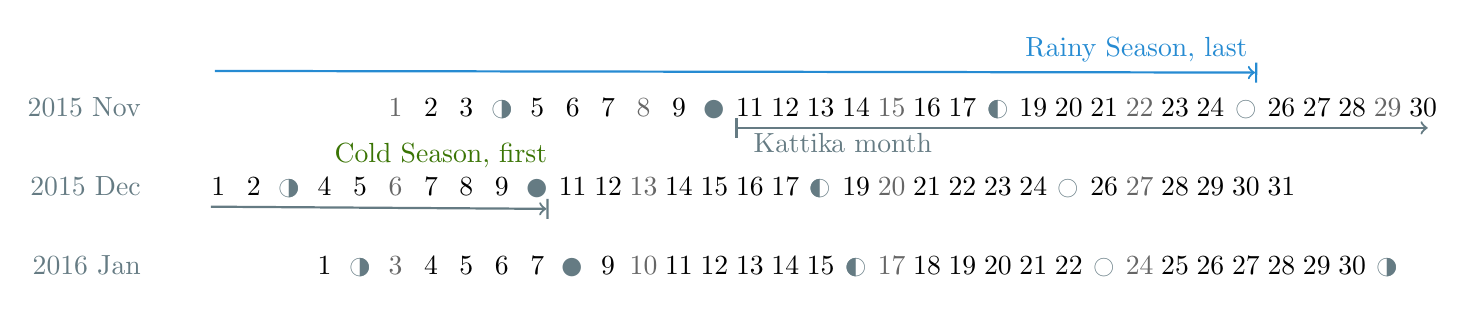
\begin{tikzpicture}[
    cold-interval-line/.style={ draw=green },
    cold-label/.style={ color=green },
    rainy-interval-line/.style={ draw=blue },
    rainy-label/.style={ color=blue },
  ]

\calendar (cal) [dates=2015-11-01 to 2016-01-31, planner] \moondays;
\node [rainy-label, above left=7pt and 0pt of cal-2015-11-25.north east, anchor=south east] {Rainy Season, last};

\node (katt-a) [below left=-3pt and 0pt of cal-2015-11-11.south west] {};
\node (katt-b) [below=-3pt of cal-2015-11-30.south east] {};
\node (katt-c) [below left=-3pt and 0pt of cal-2015-12-01.south west] {};
\node (katt-d) [below right=-3pt and 0pt of cal-2015-12-10.south east] {};

\draw [primary-content, thick, |->] (katt-a) -- (katt-b); 
\draw [primary-content, thick, ->|] (katt-c) -- (katt-d);

\node[primary-content, below right=-1pt and 3pt of cal-2015-11-11.south west] {Kattika month};

\node (rainy-a) [above left=3pt and 68pt of cal-2015-11-01.north east] {};
\node (rainy-b) [above right=3pt and 0pt of cal-2015-11-25.north east] {};

\draw [rainy-interval-line, thick, ->|] (rainy-a) -- (rainy-b); 

\node [cold-label, above left=-3pt and -3pt of cal-2015-12-10.north east, anchor=south east] {Cold Season, first};

%\node [primary-content, below=-3pt of cal-2015-11-25.south, anchor=north] {Kattika New Moon};
%\node [primary-content, below=-3pt of cal-2015-12-10.south, anchor=north] {Kattika New Moon};
\end{tikzpicture}%
}

\end{document}
